\documentclass{article}
\usepackage[utf8]{inputenc}
\usepackage[english]{babel}
\usepackage{url}
\usepackage{graphicx}
\usepackage{array}
\usepackage{geometry}
\usepackage{amsmath}
\usepackage{subcaption}
\usepackage{xcolor}
\usepackage{amsmath,accents}
\usepackage{physics}
\usepackage{setspace}
\usepackage{caption}
\usepackage{float}
\usepackage[makeroom]{cancel}
\usepackage{tikz}
\usepackage{multicol}
\usepackage{fancyhdr}
\usepackage{hhline}
\usepackage[authoryear,sort,round]{natbib}
\usepackage{aliascnt}
\newaliascnt{eqfloat}{equation}
\newfloat{eqfloat}{ht}{eqflts}
\floatname{eqfloat}{Equation}

\newcommand{\myvect}[1]{\accentset{\rightharpoonup}{#1}}

\bibliographystyle{plainnat}

\tikzset{every picture/.style={line width=0.75pt}}

\doublespacing
\setlength\parindent{24pt}
\allowdisplaybreaks

\begin{document}

\pagestyle{fancy}
\fancyhead[R]{}
\fancyhead[L]{}
\fancyhead[C]{\textbf{Calculating the rate of hydrolysis of acetylsalicylic acid and its change through pHs}}
\fancyfoot[L]{Chemistry Internal Assessment\\
for the International Baccalaureate Diploma}
\fancyfoot[R]{candidate number\\ student code}
\renewcommand{\headrulewidth}{0.4pt}
\renewcommand{\footrulewidth}{2pt}

\section{Introduction}
The investigation into the hydrolysis of acetylsalicylic acid, known as aspirin, across different ph conditions aims to quantity its degradation rate, a critical factor for the pharmaceutical's stability, shelf life, and effectiveness. The focus on hydrolysis, recognized as a first-order reaction, offers insights into the compound's behavior in aqueous solutions, relevant to both storage and physiological effects. The personal significance comes from the uncertainty that comes with ingesting aspirin, especially in how long can you wait until it becomes ineffective. The idea that it can react with water is unintuitive for me, raising intrigue in how fast it does, and at what rate.

The overarching study's research question is to what extent does aspirin (acetylsalicylic acid) stays medically relevant, and how the pH of the medium influences its hydrolysis. The conversion of acetylsalicylic acid into salicylic acid, alongside the interaction of the hydrolysis products with iron(Ill) nitrate for spectrophotometric analysis are the relevant chemical processes. This enables a detailed quantitative evaluation of the hydrolysis reaction over time. By varying the reaction medium's pH to 4, 7, and 10, the research explores how acid and alkaline conditions affect hydrolysis rates, therefore illuminating aspirin's kinetic properties under different environmental conditions (this paper also uses \cite{ChatGPT2023} as an aid in research and formatting).

The methodology includes a thorough evaluation of measurement and concentration uncertainties. This approach not only highlights the scientific diligence of the research but also recognizes potential errors and limitations posed by the laboratory setup. There are other experiments for the measuring of the hydrolysis of acetylsalicylic acid, but few of the ones I've read use pH as an independent variable. Not only that, but in this setup, the concentration of acetylsalicylic acid is controlled and equal, easing the analysis. These considerations are essential for the accurate interpretation of results and underscore the analysis's goal to dissect the hydrolysis process. The study however does not lack limitations. Between material accuracy, human error and lack of expertise and experience are a few of the many limits imposed on the methodology.

Moreover, this study is an introduction to the field of pharmaceutical chemistry by deepening the understanding of drug stability. Through experimentation and analysis, the outcomes are anticipated to provide significant insights into aspirin's stability in aqueous conditions. This aims to preserve the medication's potency and safety, emphasizing the practical benefits of grasping aspirin's stability across various pH levels.

%------------------------------------------------------------------------------------------------------------------------------------------------------------------------------------------------------------------------------------------------------------------------------------------------------------------------------------------------------------------------------------------------------------------------------------------------------------------------------------------------------------------------------------------------------------------------------------------------------------------------------------------------------------------------------------------------------------------------------------------------------------------------------------------------------------------------------------------------------------------------------------------------------------------------
\section{Theory}
The hydrolysis of acetylsalicylic acid, more commonly known as aspirin, is a reaction that plays a critical role in the drug's stability and effectiveness. This hydrolysis is a reaction where water breaks the ester bond in aspirin to form salicylic acid. The reaction is known to be acid-catalyzed, with the rate of hydrolysis being significantly affected by the pH level of the solution (as seen in \cite{fersht1967hydrolysis} and \cite{RCSpaperexperiment}).

Under acidic conditions, the reaction mechanism involves the protonation of the carbonyl oxygen, which increases the electrophilicity of the carbonyl carbon, facilitating its attack by water molecules. This leads to the formation of a tetrahedral intermediate which, upon reorganization, results in the breakdown of the ester linkage to yield the hydrolysis products.

In a alkaline solution, the mechanism shifts. Hydroxide ions, present in higher concentration, can act as nucleophiles that directly attack the carbonyl carbon of the ester bond. This nucleophilic acyl substitution leads to the formation of a similar tetrahedral intermediate (\cite{chembook}). However, the reaction proceeds differently from this point, eventually leading to the production of the same hydrolysis products but through a distinct pathway.

The hydrolysis reaction can be described by the following chemical equation:

\begin{eqfloat}
\begin{equation}
\mathrm{CH}_3 \mathrm{COOC}_6 \mathrm{H}_4 \mathrm{COOH}+\mathrm{H}_2 \mathrm{O} \rightarrow 3 \mathrm{HOC}_6 \mathrm{H}_4 \mathrm{COOH}+\mathrm{CH}_3 \mathrm{COOH}
\label{eq: Equation of condensed formula of hydrolysis of acetylsalicylic acid}
\end{equation}
\caption{Equation of condensed formula of hydrolysis of acetylsalicylic acid}
\end{eqfloat}

It can also be seen visually through the skeletal diagram of the equation:

\begin{figure}[H]
\centering
    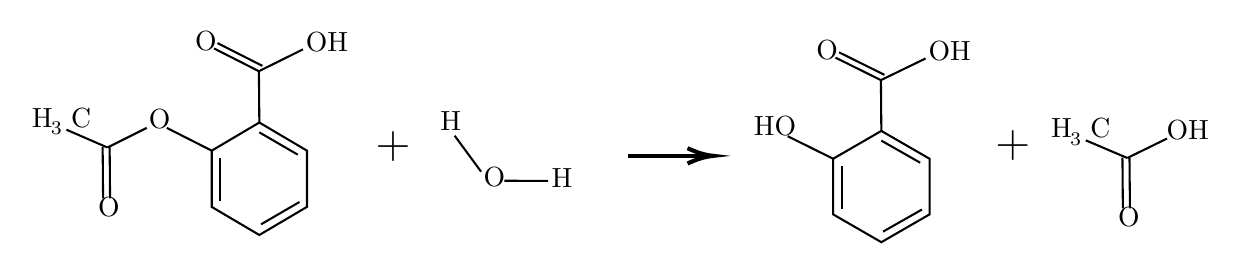
\begin{tikzpicture}[x=0.65pt,y=0.65pt,yscale=-1,xscale=1]
    \draw   (157.23,102.7) -- (130.75,118.33) -- (104.28,102.71) -- (104.28,71.44) -- (130.75,55.81) -- (157.23,71.44) -- cycle ;
    \draw    (79.31,58.79) -- (104.28,71.44) ;
    \draw    (46.31,69.7) -- (68.15,58.79) ;
    \draw    (43.64,69.46) -- (43.89,97.99) ;
    \draw    (47.53,69.46) -- (47.77,97.99) ;
    \draw    (23.5,59.78) -- (46.31,69.7) ;
    \draw    (130.75,61.27) -- (152.11,73.67) ;
    \draw    (131.72,112.38) -- (153.08,99.97) ;
    \draw    (108.92,99.48) -- (108.92,75.66) ;
    \draw    (130.51,27.28) -- (130.75,55.81) ;
    \draw    (105.55,14.62) -- (130.51,27.28) ;
    \draw    (107.49,11.65) -- (132.45,24.3) ;
    \draw    (130.51,27.28) -- (155.02,15.12) ;
    \draw    (254.04,83.13) -- (239.34,63.12) ;
    \draw    (291.25,88.24) -- (266.94,88.17) ;
    \draw   (503.33,106.87) -- (476.54,122.33) -- (449.76,106.87) -- (449.76,75.94) -- (476.54,60.47) -- (503.33,75.94) -- cycle ;
    \draw    (424.5,63.42) -- (449.76,75.94) ;
    \draw    (476.54,65.87) -- (498.15,78.15) ;
    \draw    (477.52,116.44) -- (499.13,104.17) ;
    \draw    (454.45,103.68) -- (454.45,80.11) ;
    \draw    (476.3,32.24) -- (476.54,60.47) ;
    \draw    (451.04,19.72) -- (476.3,32.24) ;
    \draw    (453.01,16.77) -- (478.26,29.29) ;
    \draw    (476.3,32.24) -- (501.09,20.21) ;
    \draw    (613.27,75.52) -- (635.36,64.71) ;
    \draw    (610.57,75.27) -- (610.81,103.5) ;
    \draw    (614.49,75.27) -- (614.74,103.5) ;
    \draw    (590.19,65.7) -- (613.27,75.52) ;
    \draw [line width=1.5]    (335.67,74.33) -- (380,74.33) ;
    \draw [shift={(383,74.33)}, rotate = 180] [color={rgb, 255:red, 0; green, 0; blue, 0 }  ][line width=1.5]    (14.21,-4.28) .. controls (9.04,-1.82) and (4.3,-0.39) .. (0,0) .. controls (4.3,0.39) and (9.04,1.82) .. (14.21,4.28)   ;
    \draw (67.6,46.82) node [anchor=north west][inner sep=0.75pt]   [align=left] {O};
    \draw (39.45,95.94) node [anchor=north west][inner sep=0.75pt]   [align=left] {O};
    \draw (2.54,46.07) node [anchor=north west][inner sep=0.75pt]   [align=left] {H \ C};
    \draw (13.16,54.06) node [anchor=north west][inner sep=0.75pt]   [align=left] {{\scriptsize 3}};
    \draw (93.32,3.65) node [anchor=north west][inner sep=0.75pt]   [align=left] {O};
    \draw (154.91,4.14) node [anchor=north west][inner sep=0.75pt]   [align=left] {OH};
    \draw (229.73,48.15) node [anchor=north west][inner sep=0.75pt]   [align=left] {H};
    \draw (253.77,79.35) node [anchor=north west][inner sep=0.75pt]   [align=left] {O};
    \draw (193.8,59.29) node [anchor=north west][inner sep=0.75pt]   [align=left] {{\LARGE +}};
    \draw (403.91,50.51) node [anchor=north west][inner sep=0.75pt]   [align=left] {HO};
    \draw (438.74,8.77) node [anchor=north west][inner sep=0.75pt]   [align=left] {O};
    \draw (501.12,9.26) node [anchor=north west][inner sep=0.75pt]   [align=left] {OH};
    \draw (538.33,58.49) node [anchor=north west][inner sep=0.75pt]   [align=left] {{\LARGE +}};
    \draw (633.43,52.79) node [anchor=north west][inner sep=0.75pt]   [align=left] {OH};
    \draw (606.4,101.39) node [anchor=north west][inner sep=0.75pt]   [align=left] {O};
    \draw (569.17,52.05) node [anchor=north west][inner sep=0.75pt]   [align=left] {H \ C};
    \draw (579.79,60.01) node [anchor=north west][inner sep=0.75pt]   [align=left] {{\scriptsize 3}};
    \draw (291.57,79.82) node [anchor=north west][inner sep=0.75pt]   [align=left] {H};
    \end{tikzpicture}
\caption{Skeletal formula of the hydrolysis of acetylsalicylic acid} 
\label{fig: Skeletal formula of the hydrolysis of acetylsalicylic acid}
\end{figure}

The subsequent reaction of salicylic acid with iron(III) nitrate is used for analytical purposes. Salicylic acid reacts with iron(III) ions to form a metallic complex that can be quantified spectrophotometrically due to its distinctive color (as seen in \cite{Studyofhydrolysisofacetylsaliciticacid}). The stoichiometry of the reaction is illustrated in the equation:

\begin{eqfloat}
\begin{equation}
3 \mathrm{HOC}_6 \mathrm{H}_4 \mathrm{COOH}+\mathrm{Fe}\left(\mathrm{NO}_3\right)_3 \rightarrow \mathrm{Fe}\left(\mathrm{C}_6 \mathrm{H}_4(\mathrm{OH}) \mathrm{COO}\right)_3+3 \mathrm{HNO}_3
\label{eq: Equation of condensed formula salicylic acid and iron(III) nitrate}
\end{equation}
\caption{Equation of condensed formula of the metathesis salicylic acid acid and iron(III) nitrate}
\end{eqfloat}

The same equation can also be illustrated through the illustration of the skeletal diagram of the reaction:

\begin{figure}[H]
\centering
    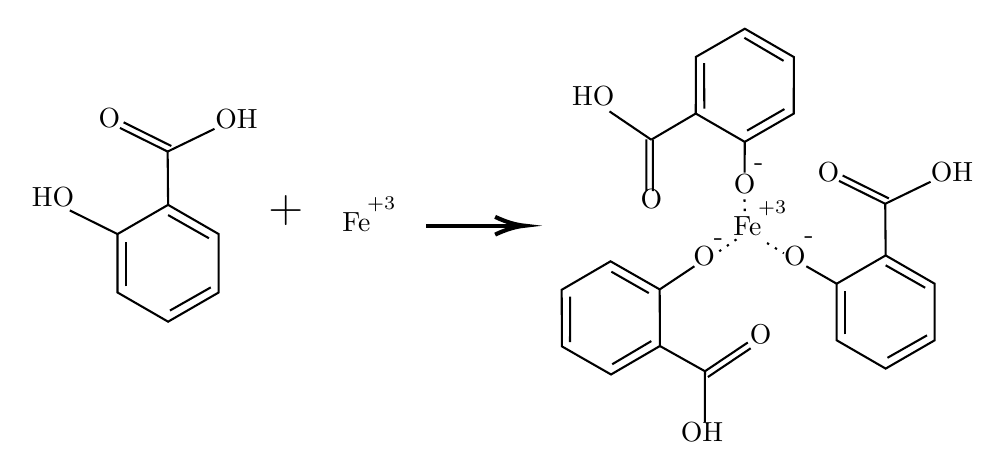
\begin{tikzpicture}[x=0.75pt,y=0.75pt,yscale=-1,xscale=1]
    \draw   (92.93,145.83) -- (68.56,159.9) -- (44.19,145.83) -- (44.19,117.69) -- (68.56,103.62) -- (92.93,117.69) -- cycle ;
    \draw    (21.22,106.3) -- (44.19,117.69) ;
    \draw    (68.56,108.54) -- (88.22,119.7) ;
    \draw    (69.46,154.54) -- (89.11,143.38) ;
    \draw    (48.46,142.93) -- (48.46,121.49) ;
    \draw    (68.34,77.94) -- (68.56,103.62) ;
    \draw    (45.36,66.55) -- (68.34,77.94) ;
    \draw    (47.15,63.87) -- (70.13,75.26) ;
    \draw    (68.34,77.94) -- (90.9,67) ;
    \draw [line width=1.5]    (193,113.67) -- (237.33,113.67) ;
    \draw [shift={(240.33,113.67)}, rotate = 180] [color={rgb, 255:red, 0; green, 0; blue, 0 }  ][line width=1.5]    (14.21,-4.28) .. controls (9.04,-1.82) and (4.3,-0.39) .. (0,0) .. controls (4.3,0.39) and (9.04,1.82) .. (14.21,4.28)   ;
    \draw   (346.42,18.75) -- (370.02,32.39) -- (370,59.65) -- (346.39,73.27) -- (322.79,59.62) -- (322.81,32.36) -- cycle ;
    \draw    (346.33,88.14) -- (346.39,73.27) ;
    \draw    (326.91,57.24) -- (326.78,35.35) ;
    \draw    (365.09,34.24) -- (346.21,23.14) ;
    \draw    (365.5,57.47) -- (347.51,67.85) ;
    \draw    (301.34,72.23) -- (322.79,59.62) ;
    \draw    (302.13,97.02) -- (302.09,72.24) ;
    \draw    (299.03,96.82) -- (298.99,72.03) ;
    \draw    (301.34,72.23) -- (281.24,58.6) ;
    \draw   (437.89,168.87) -- (414.28,182.51) -- (390.68,168.87) -- (390.68,141.61) -- (414.28,127.98) -- (437.89,141.61) -- cycle ;
    \draw    (376.04,133.21) -- (390.68,141.61) ;
    \draw    (414.28,132.74) -- (433.32,143.56) ;
    \draw    (415.15,177.31) -- (434.19,166.5) ;
    \draw    (394.81,166.06) -- (394.81,145.29) ;
    \draw    (414.07,103.1) -- (414.28,127.98) ;
    \draw    (391.81,92.07) -- (414.07,103.1) ;
    \draw    (393.54,89.47) -- (415.8,100.51) ;
    \draw    (414.07,103.1) -- (435.92,92.5) ;
    \draw   (258.3,171.81) -- (258.18,144.55) -- (281.74,130.82) -- (305.4,144.35) -- (305.52,171.62) -- (281.96,185.34) -- cycle ;
    \draw    (322.11,133.21) -- (305.4,144.35) ;
    \draw    (301.38,169.25) -- (282.54,180.41) ;
    \draw    (262.26,147.88) -- (262.2,169.78) ;
    \draw    (282.12,135.81) -- (300.16,146.12) ;
    \draw    (327.22,183.78) -- (305.52,171.62) ;
    \draw    (347.85,169.93) -- (327.22,183.78) ;
    \draw    (349.24,172.72) -- (328.62,186.57) ;
    \draw    (327.22,183.78) -- (327.13,208.38) ;
    \draw [line width=0.75]  [dash pattern={on 0.84pt off 2.51pt}]  (346.26,101.01) -- (346.48,109.87) ;
    \draw [line width=0.75]  [dash pattern={on 0.84pt off 2.51pt}]  (357.13,122.01) -- (365.22,126.95) ;
    \draw [line width=0.75]  [dash pattern={on 0.84pt off 2.51pt}]  (342.38,120.26) -- (332.91,126.81) ;
    \draw (1.4,93.84) node [anchor=north west][inner sep=0.75pt]   [align=left] {HO};
    \draw (33.59,55.87) node [anchor=north west][inner sep=0.75pt]   [align=left] {O};
    \draw (89.84,56.32) node [anchor=north west][inner sep=0.75pt]   [align=left] {OH};
    \draw (115.5,97.52) node [anchor=north west][inner sep=0.75pt]   [align=left] {{\LARGE +}};
    \draw (339.67,87.39) node [anchor=north west][inner sep=0.75pt]  [rotate=-359.98] [align=left] {O};
    \draw (294.69,94.93) node [anchor=north west][inner sep=0.75pt]  [rotate=-0.07] [align=left] {O};
    \draw (261.69,45.05) node [anchor=north west][inner sep=0.75pt]  [rotate=-0.04] [align=left] {HO};
    \draw (363.88,122.42) node [anchor=north west][inner sep=0.75pt]   [align=left] {O};
    \draw (380.03,81.87) node [anchor=north west][inner sep=0.75pt]  [rotate=-0.43] [align=left] {O};
    \draw (434.52,81.9) node [anchor=north west][inner sep=0.75pt]   [align=left] {OH};
    \draw (320.17,122.31) node [anchor=north west][inner sep=0.75pt]  [rotate=-0.19] [align=left] {O};
    \draw (347.54,159.78) node [anchor=north west][inner sep=0.75pt]  [rotate=-1.56] [align=left] {O};
    \draw (314.14,206.91) node [anchor=north west][inner sep=0.75pt]  [rotate=-0.3] [align=left] {OH};
    \draw (330.03,116.12) node [anchor=north west][inner sep=0.75pt]   [align=left] {\mbox{-}};
    \draw (373.61,115.12) node [anchor=north west][inner sep=0.75pt]   [align=left] {\mbox{-}};
    \draw (349.44,79.75) node [anchor=north west][inner sep=0.75pt]  [rotate=-0.43] [align=left] {\mbox{-}};
    \draw (339.45,107.7) node [anchor=north west][inner sep=0.75pt]   [align=left] {Fe};
    \draw (351.34,100.1) node [anchor=north west][inner sep=0.75pt]   [align=left] {{\scriptsize +3}};
    \draw (151.02,105.93) node [anchor=north west][inner sep=0.75pt]   [align=left] {Fe};
    \draw (162.91,98.34) node [anchor=north west][inner sep=0.75pt]   [align=left] {{\scriptsize +3}};
    \end{tikzpicture}
\caption{Skeletal formula of the metathesis of salicylic acid acid and iron(III) nitrate} 
\label{fig: Skeletal formula of the metathesis salicylic acid acid and iron(III) nitrate}
\end{figure}

The colored complex's absorbance at a specific wavelength is indicative of the concentration of salicylic acid present in the solution, which, in turn, reflects the extent of hydrolysis of acetylsalicylic acid under different pH conditions. The precise wavelength and the molar absorptivity coefficient of the complex are to be determined experimentally and will be discussed in the "Methodology" section. It is important to mention, that this reaction, although possible, might not be realistic. The formation of the salicitate and iron(III) metallic complex likely resembles closer to the following diagram due to the lower enthalpy required to reach the unsaturated metallic complex (as seen in \cite{campanile2016development}).

\begin{figure}[H]
\centering
    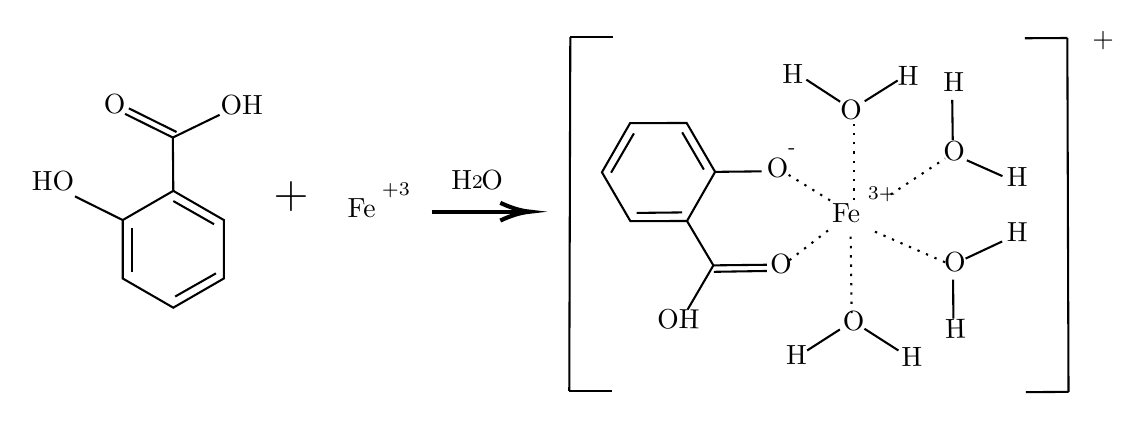
\begin{tikzpicture}[x=0.75pt,y=0.75pt,yscale=-1,xscale=1]
    %uncomment if require: \path (0,214); %set diagram left start at 0, and has height of 214
    
    %Shape: Polygon [id:dp6277584517989804] 
    \draw   (162.7,136) -- (138.33,150.07) -- (113.96,136) -- (113.96,107.86) -- (138.33,93.79) -- (162.7,107.86) -- cycle ;
    %Straight Lines [id:da40359847808214555] 
    \draw    (90.98,96.47) -- (113.96,107.86) ;
    %Straight Lines [id:da34179496650960606] 
    \draw    (138.33,98.7) -- (157.98,109.87) ;
    %Straight Lines [id:da509197674931818] 
    \draw    (139.22,144.71) -- (158.88,133.54) ;
    %Straight Lines [id:da1660378401400746] 
    \draw    (118.23,133.1) -- (118.23,111.66) ;
    %Straight Lines [id:da22308972650199832] 
    \draw    (138.11,68.11) -- (138.33,93.79) ;
    %Straight Lines [id:da39801618678559514] 
    \draw    (115.13,56.72) -- (138.11,68.11) ;
    %Straight Lines [id:da4361846696726851] 
    \draw    (116.92,54.04) -- (139.89,65.43) ;
    %Straight Lines [id:da891589275864924] 
    \draw    (138.11,68.11) -- (160.66,57.16) ;
    %Straight Lines [id:da7401950812538893] 
    \draw [line width=1.5]    (262.77,103.83) -- (307.1,103.83) ;
    \draw [shift={(310.1,103.83)}, rotate = 180] [color={rgb, 255:red, 0; green, 0; blue, 0 }  ][line width=1.5]    (14.21,-4.28) .. controls (9.04,-1.82) and (4.3,-0.39) .. (0,0) .. controls (4.3,0.39) and (9.04,1.82) .. (14.21,4.28)   ;
    %Shape: Polygon [id:dp0343773238059466] 
    \draw   (344.85,84.84) -- (358.4,61.18) -- (385.66,61.08) -- (399.37,84.64) -- (385.83,108.3) -- (358.57,108.4) -- cycle ;
    %Straight Lines [id:da9693658358923647] 
    \draw    (421.77,84.39) -- (399.37,84.64) ;
    %Straight Lines [id:da836929428817879] 
    \draw    (383.44,104.18) -- (361.54,104.42) ;
    %Straight Lines [id:da8513131363540447] 
    \draw    (360.26,66.1) -- (349.25,85.03) ;
    %Straight Lines [id:da11289610137386041] 
    \draw    (383.5,65.59) -- (393.95,83.54) ;
    %Straight Lines [id:da5652773958185833] 
    \draw    (398.54,129.69) -- (385.83,108.3) ;
    %Straight Lines [id:da31200523301411554] 
    \draw    (424.27,129.39) -- (398.41,129.69) ;
    %Straight Lines [id:da2703964349854151] 
    \draw    (424.27,132.39) -- (398.77,132.8) ;
    %Straight Lines [id:da7939257282688987] 
    \draw    (398.54,129.69) -- (386.14,150.95) ;
    %Straight Lines [id:da28703727004005086] 
    \draw [line width=0.75]  [dash pattern={on 0.84pt off 2.51pt}]  (453.77,112.89) -- (435.16,127.21) ;
    %Straight Lines [id:da2773009609769127] 
    \draw [line width=0.75]  [dash pattern={on 0.84pt off 2.51pt}]  (454.77,98.39) -- (434.16,85.71) ;
    %Straight Lines [id:da3423674168393198] 
    \draw    (471.32,160.22) -- (487.7,170.71) ;
    %Straight Lines [id:da36771527532353576] 
    \draw    (443.7,170.71) -- (459.49,160.57) ;
    %Straight Lines [id:da2232138625797485] 
    \draw    (459.63,50.85) -- (443.34,40.22) ;
    %Straight Lines [id:da5257396898893] 
    \draw    (487.34,40.61) -- (471.46,50.61) ;
    %Straight Lines [id:da6468243609960391] 
    \draw    (520.06,126.42) -- (537.68,118.17) ;
    %Straight Lines [id:da7877776045993174] 
    \draw    (514.17,155.36) -- (514.04,136.6) ;
    %Straight Lines [id:da12927361023718564] 
    \draw    (513.87,69.38) -- (513.62,49.93) ;
    %Straight Lines [id:da8351956968355503] 
    \draw    (537.81,86.69) -- (520.66,79.07) ;
    %Straight Lines [id:da8524635893353822] 
    \draw [line width=0.75]  [dash pattern={on 0.84pt off 2.51pt}]  (510.16,128.21) -- (474.02,112.42) ;
    %Straight Lines [id:da3304516471435892] 
    \draw [line width=0.75]  [dash pattern={on 0.84pt off 2.51pt}]  (465.16,152.71) -- (464.66,113.71) ;
    %Straight Lines [id:da44127819601086005] 
    \draw [line width=0.75]  [dash pattern={on 0.84pt off 2.51pt}]  (466.16,98.21) -- (466.16,59.21) ;
    %Straight Lines [id:da7912950911126325] 
    \draw [line width=0.75]  [dash pattern={on 0.84pt off 2.51pt}]  (484,95.5) -- (510.16,78.21) ;
    %Straight Lines [id:da05657151572721042] 
    \draw    (329.61,19.71) -- (329.11,190.21) ;
    %Straight Lines [id:da9674930647097559] 
    \draw    (349.61,190.21) -- (329.11,190.21) ;
    %Straight Lines [id:da7128008198092544] 
    \draw    (350.11,19.71) -- (329.61,19.71) ;
    %Straight Lines [id:da0609589416451507] 
    \draw    (569.64,190.64) -- (569.07,20.14) ;
    %Straight Lines [id:da5414777940139852] 
    \draw    (548.57,20.27) -- (569.07,20.14) ;
    %Straight Lines [id:da7137774822964449] 
    \draw    (549.14,190.77) -- (569.64,190.64) ;
    
    % Text Node
    \draw (68.67,83) node [anchor=north west][inner sep=0.75pt]   [align=left] {HO};
    % Text Node
    \draw (103.36,46.04) node [anchor=north west][inner sep=0.75pt]   [align=left] {O};
    % Text Node
    \draw (159.61,46.48) node [anchor=north west][inner sep=0.75pt]   [align=left] {OH};
    % Text Node
    \draw (185.27,87.68) node [anchor=north west][inner sep=0.75pt]   [align=left] {{\LARGE +}};
    % Text Node
    \draw (422.68,76.71) node [anchor=north west][inner sep=0.75pt]  [rotate=-359.29] [align=left] {O};
    % Text Node
    \draw (424.39,122.87) node [anchor=north west][inner sep=0.75pt]  [rotate=-359.38] [align=left] {O};
    % Text Node
    \draw (370.1,149.41) node [anchor=north west][inner sep=0.75pt]  [rotate=-1.08] [align=left] {OH};
    % Text Node
    \draw (454.22,98.36) node [anchor=north west][inner sep=0.75pt]   [align=left] {Fe};
    % Text Node
    \draw (220.79,96.1) node [anchor=north west][inner sep=0.75pt]   [align=left] {Fe};
    % Text Node
    \draw (237.34,88.51) node [anchor=north west][inner sep=0.75pt]   [align=left] {{\scriptsize +3}};
    % Text Node
    \draw (270.77,82.67) node [anchor=north west][inner sep=0.75pt]   [align=left] {H O};
    % Text Node
    \draw (280.67,85.01) node [anchor=north west][inner sep=0.75pt]   [align=left] {{\scriptsize 2}};
    % Text Node
    \draw (432.14,166.98) node [anchor=north west][inner sep=0.75pt]  [rotate=-359.96] [align=left] {H};
    % Text Node
    \draw (487.67,167.6) node [anchor=north west][inner sep=0.75pt]  [rotate=-359.36] [align=left] {H};
    % Text Node
    \draw (459.39,150.51) node [anchor=north west][inner sep=0.75pt]  [rotate=-359.98] [align=left] {O};
    % Text Node
    \draw (498.87,44.45) node [anchor=north west][inner sep=0.75pt]  [rotate=-180.47] [align=left] {H};
    % Text Node
    \draw (443.34,43.32) node [anchor=north west][inner sep=0.75pt]  [rotate=-179.87] [align=left] {H};
    % Text Node
    \draw (471.47,60.67) node [anchor=north west][inner sep=0.75pt]  [rotate=-180.49] [align=left] {O};
    % Text Node
    \draw (508.65,154.45) node [anchor=north west][inner sep=0.75pt]  [rotate=-358.93] [align=left] {H};
    % Text Node
    \draw (538.58,107.57) node [anchor=north west][inner sep=0.75pt]  [rotate=-0.59] [align=left] {H};
    % Text Node
    \draw (508.22,122.08) node [anchor=north west][inner sep=0.75pt]  [rotate=-0.05] [align=left] {O};
    % Text Node
    \draw (538.39,81.01) node [anchor=north west][inner sep=0.75pt]  [rotate=-359.78] [align=left] {H};
    % Text Node
    \draw (507.85,35.19) node [anchor=north west][inner sep=0.75pt]  [rotate=-0.18] [align=left] {H};
    % Text Node
    \draw (507.95,68.33) node [anchor=north west][inner sep=0.75pt]  [rotate=-0.24] [align=left] {O};
    % Text Node
    \draw (579.61,15.67) node [anchor=north west][inner sep=0.75pt]   [align=left] {+};
    % Text Node
    \draw (471.51,90.34) node [anchor=north west][inner sep=0.75pt]   [align=left] {{\scriptsize 3+}};
    % Text Node
    \draw (433,70.5) node [anchor=north west][inner sep=0.75pt]  [font=\scriptsize] [align=left] {\mbox{-}};
    
    
\end{tikzpicture}
\caption{Skeletal formula of the metathesis of salicylic acid acid and iron(III) nitrate (unsaturated)} 
\label{fig: Skeletal formula of the metathesis salicylic acid acid and iron(III) nitrate (unsaturated)}
\end{figure}

These theoretical considerations form the basis for the experimental approach, which involves adjusting the pH of the solution and monitoring the change in concentration of the hydrolysis product over time. It is empirical to also understand that temperature plays a role in this reaction, however, it will not be a variable in our case. The experiment aims to explore the intrinsic chemical properties of aspirin and the impact of pH on its stability. The anticipated data will provide insight into the optimal conditions for the storage and use of aspirin, with implications for its formulation and shelf life.

%--------------------------------------------------------------------------------------------------------------------------------------------------------------------------------------------------------------------------------------------------------------------
\section{Methodology}

The procedure to measure the hydrolysis rate of acetylsalicylic acid employs a spectrophotometer for analysis. The methodology follows a series of steps to prepare the reaction mixture and analyze its components over time, and heavily inspired by \cite{RCSpaperexperiment}, but adapted to accommodate the change in pH and analysis of the rate.

\subsection{Materials and Apparatus}
\begin{multicols}{2}
\begin{itemize}
    \item Visible light spectrophotometer ($\pm$0.1AU)
    \item Spectrophotometer cuvettes that can hold 6 $\text{cm}^3$
    \item 5 $\text{cm}^3$ and 1 $\text{cm}^3$ volumetric pipettes ($\pm$0.01$\text{cm}^3$)
    \item Powdered acetylsalicylic acid
    \item 50ml of $0.025$ mol $\text{cm}^3$ iron(III) chloride ($\pm0.01\text{cm}^3$)
    \item 250ml of 4pH, 7pH, 10pH buffer solutions
    \item 3 thermometer ($\pm$0.5ºC)
    \item 3 conical flasks of 100 $\text{cm}^3$ ($\pm$0.1$\text{cm}^3$)
    \item 3 beakers of 100 $\text{cm}^3$ ($\pm$0.1$\text{cm}^3$)
    \item 3 graduated cylinders of 100 $\text{cm}^3$ ($\pm$0.1$\text{cm}^3$)
    \item Hot plate magnetic stirrers
    \item Stir bar (or flea)
    \item Digital balance of max 120g ($\pm$0.001g)
\end{itemize}
\end{multicols}

\begin{figure}[H]
\centering
\includegraphics[width=0.9\textwidth]{img/Big setup.jpg}
\caption{Experimental Setup}
\label{fig:experimental setup}
\end{figure}

Due to the short time in between measurements during the procedure, the setup should be prepared accordingly, making sure to keep efficient as not to introduce time discrepancies in the measurements. The figure above shows how this could be done. The uncertainty of the powdered acetylsalicylic acid and buffer solution is considered are both considered to be equal to zero.

\subsection{Health and Safety}
Wear eye protection throughout the experimental process to protect against chemical splashes and heat. Gloves and lab coats are also necessary as high and low pHs are involved. Remaining material and mixtures are to be properly disposed of.

\subsection{Procedure}
Heat 100$\text{cm}^3$ of the buffer solution to 70 °C in a conical flask on a magnetic stirrer/hotplate. Introduce a magnetic flea to ensure uniform stirring of the solution. Measure 0.10g of powdered acetylsalicylic acid and add it to the flask. Stir until the solid dissolves completely. Do not record any measurements until the powdered acetylsalicylic acid is completely dissolved.

Prepare a mixture for spectrophotometric analysis by combining iron(III) nitrate reagent with a sample of the reaction solution in a visible light spectorophotometer tube. A solution of 5$\text{cm}^3$ of the iron(III) nitrate and 1$\text{cm}^3$ of the solution should be used in the spectrophotometer analysis. Measure the absorbance of the mixture to gauge the concentration of the salicitate and iron(III) metallic complex. 

Collect samples from the reaction mixture every 15 minutes and repeat the absorbance measurement for each. Converting the absorbance data to concentrations using a predetermined calibration graph is not necessary as the rate can be quantified without it. Introducing concentration will only introduce uncertainty.

To examine the influence of pH on hydrolysis, replicate the experiment with buffer solutions at different pH levels. This can be done sequentially or parallelly depending on the amount of time available.

%--------------------------------------------------------------------------------------------------------------------------------------------------------------------------------------------------------------------------------------------------------------------
\section{Data}

This section presents the results of the spectrophotometric analysis, showing how the absorbance at 580nm changes over time during the hydrolysis of acetylsalicylic acid under different pH conditions. The data is illustrated through a spectrum graph and a line graph with corresponding trendlines for each pH level. The uncertainty of the section includes solely the uncertainty for the light spectrophotometer, and the molarity of the reactants are irrelevant. Due to the fact that the desired measurement is the rate, and the same solution of acetylsalicylic acid is used for each test makes the value of the molarity irrelevant when it comes to rate. Similarly, the iron(III) complex is not the limiting reagent, and therefore its uncertainty is irrelevant. The values of the light spectrophotometer is mentioned in the materials and apparatus section.

The spectrometer absorbance graph displays the full spectrum of wavelengths measured during the experiment. Peaks in this graph indicate the presence of hydrolysis products at various pH levels.

\begin{figure}[H]
\centering
\includegraphics[width=0.9\textwidth]{img/Chem Graph IA.png}
\caption{Spectrometer absorbance graph}
\label{fig:Spectrometer absorbance graph}
\end{figure}

The following table lists absorbance values at 580nm, a wavelength chosen for its relevance to the metallic complex absorption peak.

\begin{table}[!ht]
    \centering
    \begin{tabular}{|l|l|l|l|}
    \hline
        Time (minutes) & \multicolumn{2}{l}{Absorbance at 580nm (AU)} & \\ \hline
        pH of buffer solution & pH 4 \enspace \enspace \enspace \enspace \enspace \enspace & pH 7 & pH 10 \enspace \enspace \enspace \enspace \enspace \enspace \\ \hhline{|=|=|=|=|}
        0 & 0.2$\pm$0.1 & 0.1$\pm$0.1 & 0.5$\pm$0.1 \\ \hline
        15 & 0.5$\pm$0.1 & 0.7$\pm$0.1 & 0.8$\pm$0.1 \\ \hline
        30 & 0.5$\pm$0.1 & 0.7$\pm$0.1 & 0.8$\pm$0.1 \\ \hline
        45 & 0.6$\pm$0.1 & 0.8$\pm$0.1 & 0.9$\pm$0.1 \\ \hline
        60 & 0.7$\pm$0.1 & 0.9$\pm$0.1 & 0.9$\pm$0.1 \\ \hline
        75 & 0.7$\pm$0.1 & 1.0$\pm$0.1 & 0.9$\pm$0.1 \\ \hline
    \end{tabular}
\end{table}

Next, the scatter plot visualizes the rate of hydrolysis reaction over time for each pH level, providing a view of how reaction rates compare across the pH scale.

\begin{figure}[H]
\centering
\includegraphics[width=0.9\textwidth]{img/Chem IA graph rate.png}
\caption{Graph of the absorbance of the solution through time at 580nm with trendlines}
\label{fig:Graph of the absorbance of the solution through time at 580nm with trendlines}
\end{figure}

These data sets provide a simple mathematical representation of the hydrolysis reaction rates under various pH conditions. It should also be mentioned that the uncertainty of the molarity for the acetylsalicylic acid is irrelevant compared to the uncertainty for the light spectrophotometer.
A change in color of the solution can also be seen, showing a change in chemical structure of the mixture. Although not always a significant change in color, the same can easily be noticed. Previous samples left untouched also go through a change in color, showing furthermore that time is an aspect of the reaction.

%------------------------------------------------------------------------------------------------------------------------------------------------------------------------------------------------------------------------------------------------------------------------------------------------------------------------------------------------------------------------------------------------------------------------------------------------------------------------------------------------------------------------------------------------------------------------------------------------------------------------------------------------------------------------------------------------------------------------------------------------------------------------------------------------------------------------------------------------------------------------------------------------------------------------
\section{Analysis}

The data values derived from the spectrophotometric data provide little insight into the rates of hydrolysis of acetylsalicylic acid under different pH conditions.

The values derived from the spetrophotometry have been turned into rates for each point through the formula $\frac{\Delta \text{absorbance at 580nm}}{\Delta \text{time}}$, and the relative uncertainty of the absorbance has been doubled since we calculate the difference by subtracting two values of absorbance. By multiplying it with the rate, we achieve the proper uncertainty. What follows is the table with improper significant figures.

\begin{table}[H]
    \centering
    \begin{tabular}{|l|l|l|l|}
    \hline
        Time (minutes) & \multicolumn{2}{l}{Rate of the hydrolysis of acetysalicylic acid (AU s$^{-1}$)}& \\ \hline
        ph & 4 \enspace\enspace\enspace\enspace\enspace\enspace\enspace\enspace\enspace\enspace\enspace\enspace\enspace\enspace\enspace\enspace& 7 & 10\enspace\enspace\enspace\enspace\enspace\enspace\enspace\enspace\enspace\enspace\enspace\enspace\enspace\enspace\enspace\enspace \\ \hline
        0 to 15 & 0.014$\pm0.01$ & 0.0407$\pm0.01$ & 0.0222$\pm0.01$ \\ \hline
        15 to 30 & 0.0033$\pm0.01$ & 0.0055$\pm0.01$ & 0.0012$\pm0.01$ \\ \hline
        30 to 45 & 0.0093$\pm0.01$ & 0.0042$\pm0.01$ & 0.0021$\pm0.01$ \\ \hline
        45 to 60 & 0.0028$\pm0.01$ & 0.0056$\pm0.01$ & 0.0009$\pm0.01$ \\ \hline
        60 to 75 & 0.0024$\pm0.01$ & 0.0032$\pm0.01$ & 0.0011$\pm0.01$ \\ \hline
        75 to 90 & 0.0007$\pm0.01$ & 0.002$\pm0.01$ & 0.0024$\pm0.01$ \\ \hline
    \end{tabular}
\end{table}

The initial low concentration of the metallic complex observed in the first measurement for pH 7 suggests an anomaly, potentially due to experimental timing or the rapid initial reaction rate at neutral pH. At pH 7, the solution facilitates a balanced hydrolysis process, possibly allowing for a more complete and immediate reaction of acetylsalicylic acid to its hydrolysis products before stabilizing to a steady rate, as reflected in the higher slope of the trendline.

In contrast, the reaction at pH 4, despite having a relatively high rate indicated by its trendline equation, may be influenced by the protonation of the carboxyl group on the salicylic acid, forming a more stable intermediate that slows down the initial formation of the iron(III)-salicylate complex. This could explain why, after the initial phase, the reaction continues at a steady but slower rate compared to the neutral pH.

For the alkaline condition at pH 10, the lower rate of reaction as indicated by the trendline slope suggests that the hydroxide ions may initially react with the acetylsalicylic acid or the hydrolysis product, salicylic acid, forming species that do not readily form the colored complex with iron(III) ions. This reaction pathway could lead to a slower overall formation of the detectable complex, contributing to the observed lower rate of hydrolysis under alkaline conditions.

The observed discrepancies and the overall reaction rates align with the theoretical understanding that the hydrolysis of acetylsalicylic acid is influenced by the pH of the solution, which affects the stability and reactivity of the hydrolysis products. The initial low concentration of the metallic complex at pH 7 and the varying rates across the pH spectrum highlight the complex dynamics of the hydrolysis reaction, suggesting that both the reaction conditions and the timing of measurements are crucial for capturing the reaction kinetics.

This however is completely insignificant due to the present uncertainty. If analysing the data with its uncertainty, the data set becomes null.

\begin{table}[H]
    \centering
    \begin{tabular}{|l|l|l|l|}
    \hline
        Time (minutes) & \multicolumn{2}{l}{Rate of the hydrolysis of acetysalicylic acid (AU s$^{-1}$)}& \\ \hline
        ph & 4\enspace\enspace\enspace\enspace\enspace\enspace\enspace\enspace\enspace\enspace\enspace\enspace\enspace\enspace\enspace\enspace & 7 & 10\enspace\enspace\enspace\enspace\enspace\enspace\enspace\enspace\enspace\enspace\enspace\enspace\enspace\enspace\enspace\enspace \\ \hline
        0 to 15 & 0.01$\pm0.01$ & 0.04$\pm0.01$ & 0.02$\pm0.01$ \\ \hline
        15 to 30 & 0.00$\pm0.01$ & 0.01$\pm0.01$ & 0.00$\pm0.01$ \\ \hline
        30 to 45 & 0.00$\pm0.01$ & 0.00$\pm0.01$ & 0.00$\pm0.01$ \\ \hline
        45 to 60 & 0.00$\pm0.01$ & 0.01$\pm0.01$ & 0.00$\pm0.01$ \\ \hline
        60 to 75 & 0.00$\pm0.01$ & 0.00$\pm0.01$ & 0.00$\pm0.01$ \\ \hline
        75 to 90 & 0.00$\pm0.01$ & 0.00$\pm0.01$ & 0.00$\pm0.01$ \\ \hline
    \end{tabular}
\end{table}

In conclusion, the analysis of the hydrolysis rates of acetylsalicylic acid under varying pH conditions shows the influence of pH on the reaction. However, due to the uncertainty of the light spectrophotometer, the data is utterly useless and no relation between pH and rate of hydrolysis can be made. Furthermore, the data with its uncertainty shows little proof of reaction at all.

%--------------------------------------------------------------------------------------------------------------------------------------------------------------------------------------------------------------------------------------------------------------------
\section{Evaluation}
The study on the hydrolysis of acetylsalicylic acid under various pH conditions highlights key areas for methodological improvement and acknowledges the strengths in its approach to data comparison. A significant limitation identified was the consistency in timing for measurements. This issue was particularly noticeable with the unexpectedly low concentration of the metallic complex in the initial measurement at pH 7, indicating that the sampling intervals might not have adequately captured the swift initial changes in the reaction rates.

Another concern was temperature stability during the experiment. The method employed did not include a means to precisely regulate temperature, which could lead to variations affecting the reaction rate and, consequently, the reliability of the collected data.

Despite these limitations, the study's design allows for a reliable comparison of values across different pH levels if it were not for the uncertainty of the light spectrophotometer. The data collected is of little use and shows little relation with proper uncertainty measurements applied to it.

Through the use of a more precise light spectrophotometer, a better relation could've been built. This is single-handedly the biggest issue of the experiment.

%--------------------------------------------------------------------------------------------------------------------------------------------------------------------------------------------------------------------------------------------------------------------
\section{Conclusion}
The investigation into the hydrolysis of acetylsalicylic acid revealed little insights into the reaction's dependency on pH levels. With no uncertainty, pH 7 showed the highest rate of reaction followed by pH 4 and then pH 10, the study underscores the significant influence of the reaction medium on the hydrolysis process. These findings are in line with theoretical expectations, where the neutral condition favors the hydrolysis of aspirin, potentially due to a more balanced interaction between the aspirin molecule and the water molecules. This conclusion however cannot be made nor evaluated since the uncertainty of the measurements are above any significant measurements.

It is a shame that the culmination of the research, creation of methodology, data measuring and processing culminated in a non-too-subtle failure. This however proves further the relevance of uncertainty not only when treating data, but especially when planning an experiment.

For future studies, improvements such as the use of a temperature-controlled heater could reduce uncertainty related to temperature variations, enhancing the precision of the reaction rate measurements. Additionally, extending the duration between measurements or employing a more detailed method to analyze the solution immediately after mixing could provide a clearer picture of the initial reaction dynamics and most importantly the use of a more precise light spectrophotometer. These adjustments would likely mitigate some of the observed weaknesses, leading to more accurate and reliable data on the hydrolysis of acetylsalicylic acid.

%--------------------------------------------------------------------------------------------------------------------------------------------------------------------------------------------------------------------------------------------------------------------
\pagebreak

\bibliography{references}

\end{document}